\documentclass[UTF8]{article}
\usepackage{graphicx}
\usepackage{subfigure}
\usepackage{amsmath}
\usepackage{makecell}
\usepackage[utf8]{inputenc}
\usepackage[space]{ctex} %中文包
\usepackage{listings} %放代码
\usepackage{xcolor} %代码着色宏包
\usepackage{CJK} %显示中文宏包
\usepackage{float}


\definecolor{mygreen}{rgb}{0,0.6,0}
\definecolor{mygray}{rgb}{0.5,0.5,0.5}
\definecolor{mymauve}{rgb}{0.58,0,0.82}
\lstset{
	backgroundcolor=\color{white}, 
	basicstyle = \footnotesize,       
	breakatwhitespace = false,        
	breaklines = true,                 
	captionpos = b,                    
	commentstyle = \color{mygreen}\bfseries,
	extendedchars = false,             
	frame =shadowbox, 
	framerule=0.5pt,
	keepspaces=true,
	keywordstyle=\color{blue}\bfseries, % keyword style
	language = Verilog,                     % the language of code
	otherkeywords={string}, 
	numbers=left, 
	numbersep=5pt,
	numberstyle=\tiny\color{mygray},
	rulecolor=\color{black},         
	showspaces=false,  
	showstringspaces=false, 
	showtabs=false,    
	stepnumber=1,         
	stringstyle=\color{mymauve},        % string literal style
	tabsize=4,          
	title=\lstname                      
}


\title{中国科学技术大学计算机学院\\《数字电路实验》报告}
\author{}

\date{}

\begin{document}
	\maketitle
	\begin{figure}[H]
		\centering
		
\includegraphics[width=2.5in]{xiaohui.jpg}\vspace{0.5cm}\\
		\large{
			实验题目:简单组合逻辑电路\\
			学生姓名:王章瀚\\
			学生学号:PB18111697\\
			完成日期:2019/10/8\\
		}\vspace{2cm}
		
		\large{计算机实验教学中心制\\2019年09月\\}
		\thispagestyle{empty}
		\clearpage  % 清除当页页码
	\end{figure}


	\section{实验目的}
	熟练掌握Logisim的基本用法\par
	进一步熟悉Logisim更多功能\par
	用Logisim设计组合逻辑电路并进行仿真\par
	初步学习Verilog语法\par
	
	\section{实验环境}
	PC 一台\par
	Windows 或 Linux 操作系统\par
	Java 运行环境(jre)\par
	Logisim 仿真工具\par
	vlab.ustc.edu.cn (jre 和 Logisim 工具都可在此网站获取)\par
	
	\section{实验过程}
	\subsection{用真值表自动生成电路}
	由于上一次实验对Logisim的操作需要大量的拖拽、布局、连线等操作,费时费力。故这次实验,学习了通过真值表生成电路的方法。\par
	实验指导书中给出了按以下真值表完成本项实验的步骤\par。
	\begin{figure}[H]
		\centering
		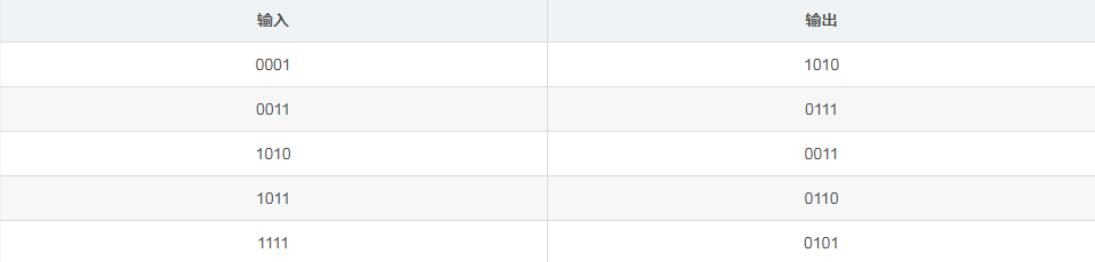
\includegraphics[scale=0.4]{BoolList.jpg}
		\caption{真值表}
		\label{BoolList}
	\end{figure}\par
	按照指导书的步骤,填写好真值表:\par
	\begin{figure}[H]
		\centering
		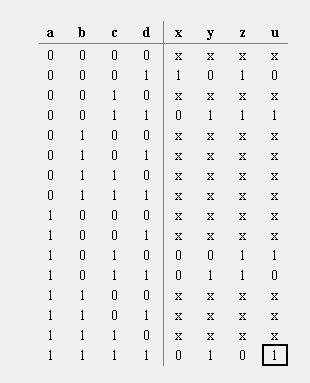
\includegraphics[scale=0.7]{FillingBoolTable.jpg}
		\caption{Logisim中填写的真值表}
		\label{FillingBoolTable}
	\end{figure}\par
	得到电路图如下:\par
	\begin{figure}[H]
		\centering
		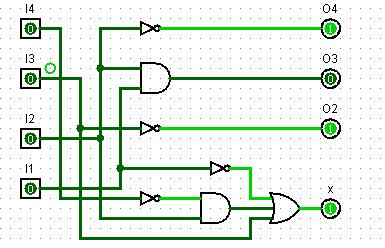
\includegraphics[scale=0.7]{CurcuitGenerateByBoolTable.jpg}
		\caption{通过真值表生成的电路}
		\label{CurcuitGenerateByBoolTable}
	\end{figure}\par
	
	\subsection{用表达式生成电路图}
	用真值表生成电路图虽然能减少工作,但是一旦输入变量变多,真值表的编辑也将成为十分麻烦的事情。但如果我们可以通过表达式来生成电路,将会使事情变得十分简单。\par
	我们可以在同样的地方选择Expression选项,填写每个输出信号的表达式,以此生成电路。\par
	我们甚至可以用Minimized选项卡对表达式进行化简,从而减少逻辑门数量。\par
	\begin{figure}[H]
		\begin{minipage}[H]{0.45\linewidth}
			\centering
			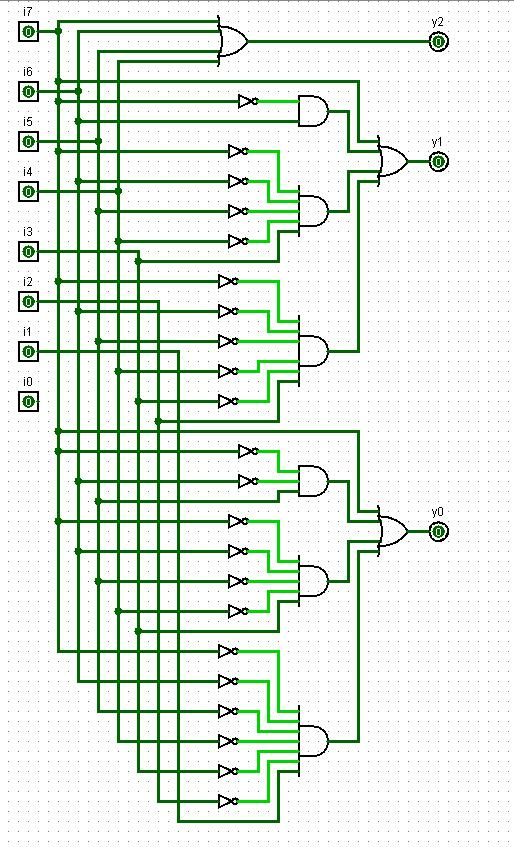
\includegraphics[scale=0.45]{CurcuitGenerateByExpression_Complex.jpg}
			\caption{未经简化的电路图}
			\label{CurcuitGenerateByExpression_Complex}
		\end{minipage}
		\begin{minipage}[H]{0.6\linewidth}
			\centering
			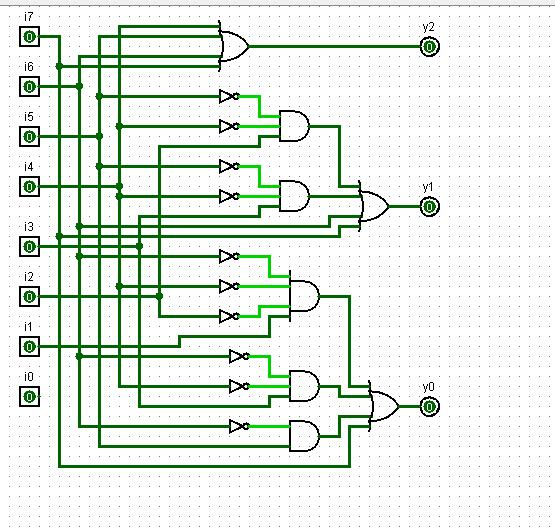
\includegraphics[scale=0.4]{CurcuitGenerateByExpression_Simple.jpg}
			\caption{经简化的电路图}
			\label{CurcuitGenerateByExpression_Simple}
		\end{minipage}
	\end{figure}
	此外,我们还可以获取电路图的信息。\par
	\begin{figure}[H]
		\centering
		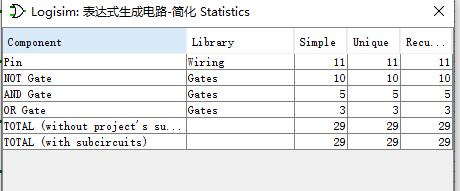
\includegraphics[scale=0.7]{getInfor.jpg}
		\caption{电路图信息}
		\label{getInfor}
	\end{figure}
	Logisim的自动生成电路功能十分方便,但也有一点不足,就是它的输入输出信号必须是单bit位宽的。\par

	\subsection{Verilog HDL语法入门}
	下面我们通过对照 Logisim 中设计的简单电路来学习Verilog语法\\
	
	\subsubsection*{例1.}如下图所示,左侧为电路结构,右侧为电路封装图,可以看到,该电路包含一个输入,取名为 in 信号(信号可自行命名),两个输出,out信号与输入直连, out\_n 信号为输入信号取反,该电路模块我们命名为test。\par
	\begin{figure}[H]
		\begin{minipage}[H]{0.45\linewidth}
			\centering
			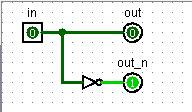
\includegraphics[scale=1]{CurcuitTest.jpg}
			\caption{test的电路图}
			\label{CurcuitTest}
		\end{minipage}
		\begin{minipage}[H]{0.6\linewidth}
			\centering
			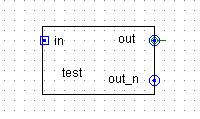
\includegraphics[scale=1]{ModuleTest.jpg}
			\caption{test的封装}
			\label{ModuleTest}
		\end{minipage}
	\end{figure}\par
	按此图,写出Verilog模块代码如下:\par
	\begin{lstlisting}[language=Verilog]
	module test(	//模块名称
		input in,	//输入信号声明
		output out,	//输出信号声明
		output out_n);
	//可在此声明内部变量
	/*******以下为逻辑描述部分******/
		assign out = in;
		assign out_n = ~in;
	/*******逻辑描述部分结束******/
	endmodule   //模块名结束关键词
	\end{lstlisting}
	
	\subsubsection*{例2.}下图左侧为半加器电路结构图,右侧为电路封装图\par
	\begin{figure}[H]
		\centering
		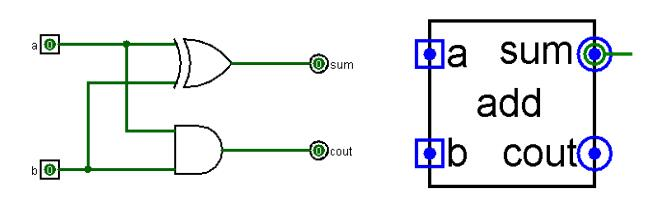
\includegraphics[scale=0.7]{half-adder.jpg}
		\label{half-adder}
	\end{figure}\par
	按此图,写出Verilog模块代码如下:\par
	\begin{lstlisting}[language=Verilog]
	module add(
		input a,b,
		output sum,cout);
		assign {cout,sum} = a + b;
	endmodule
	\end{lstlisting}\par
	这里使用了位拼接功能。其中a+b使得a和b在一起组成了一个两bit位宽的信号。而cout和sum通过位拼接符\{\}将两个单bit信号拼接成2bit信号,用于接收结果。\par
	上述代码是从行为级上描述的,效果与下面这段一样。两条赋值语句的位置是不影响结果的。
	\begin{lstlisting}[language=Verilog]
	module add(
		input a,b,
		output sum,cout);
		assign cout = a & b;
		assign sum = a ^ b;
	endmodule
	\end{lstlisting}\par
	
	\subsubsection*{例3.}利用前面例子中所设计的半加器,构造一个全加器,其电路结
	构图和电路封装图如下所示\par
	\begin{figure}[H]
		\centering
		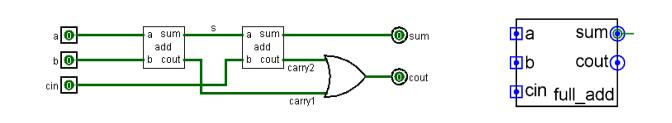
\includegraphics[scale=0.7]{adder.jpg}
		\label{adder}
	\end{figure}
	按此图,写出Verilog模块代码如下:\par
	\begin{lstlisting}[language=Verilog]
	module full_add(
		input a,b,cin,
		output sum,cout);
		wire s,carry1,carry2;
		add add_inst1(
			.a (a ),
			.b (b ),
			.sum (s ),
			.cout (carry1));
		add add_inst2(
			.a (s ),
			.b (cin ),
			.sum (sum ),
			.cout (carry2));
		assign cout = carry1 | carry2;
	endmodule
	\end{lstlisting}\par
	本例中,关键字wire表明声明的信号为线网类型,可以通过assign赋值的都是这种类型的信号。凡是没有明确声明类型的变量都被当作为线网类型wire来处理。\par
	此外,还利用到了模块调用的功能。\par
	
	
	\section{实验练习}
	
	\subsection{题目1}
	\subsubsection{题目}
	依据如下真值表,通过Logisim编辑真值表功能,完成电路设计。电路下方需标注姓名学号。\par
	\begin{figure}[h]
		\centering
		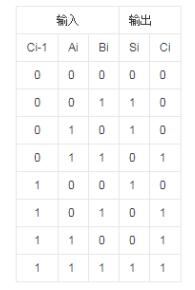
\includegraphics[scale=1]{Problem1_BoolTable.jpg}
		\label{Problem1_BoolTable}
	\end{figure}\par
	\subsubsection{实验结果}
	实验结果如下图所示:\par
	\begin{figure}[H]
		\centering
		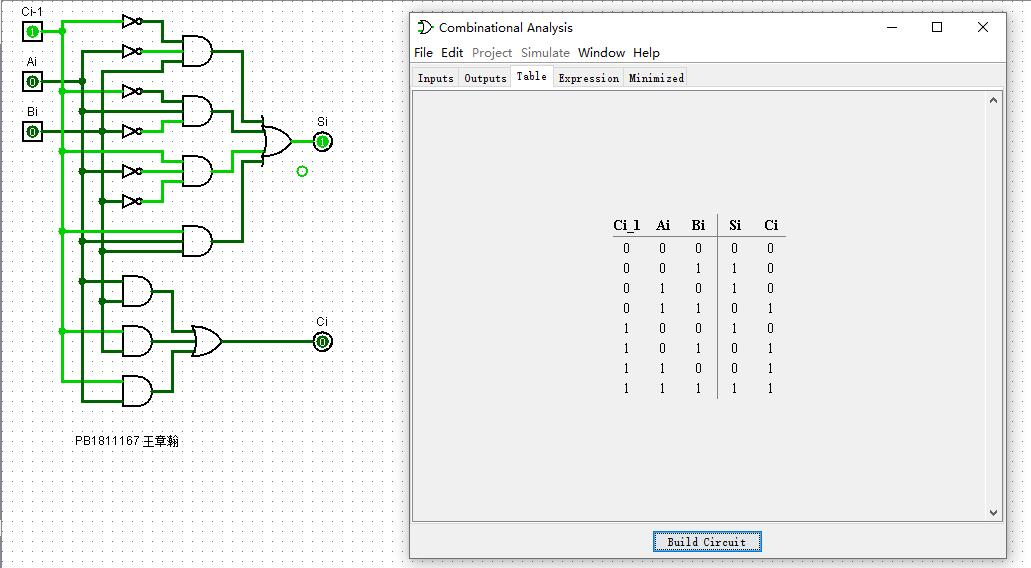
\includegraphics[scale=0.5]{Problem1.jpg}
		\caption{题目1的实验结果}
		\label{Problem1}
	\end{figure}\par

	\subsection{题目2}
	\subsubsection{题目}
	根据下列真值表,通过Logisim的编辑表达式功能完成电路设计,电路下方需标注姓名学号。\par
	\begin{figure}[h]
		\centering
		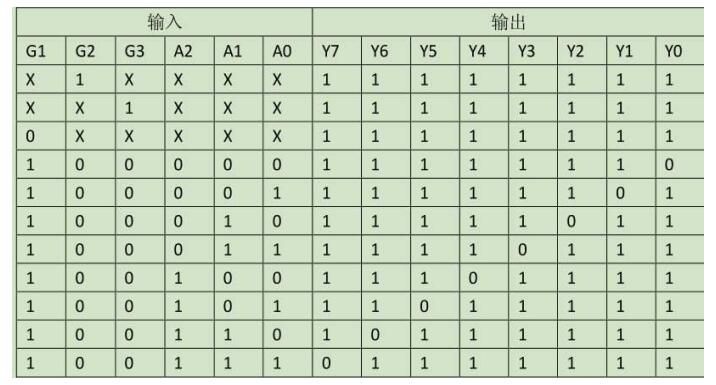
\includegraphics[scale=0.6]{Problem2_BoolTable.jpg}
		\label{Problem2_BoolTable}
	\end{figure}\par
	\subsubsection{实验结果}
	实验结果如下图所示:\par
	\begin{figure}[H]
		\centering
		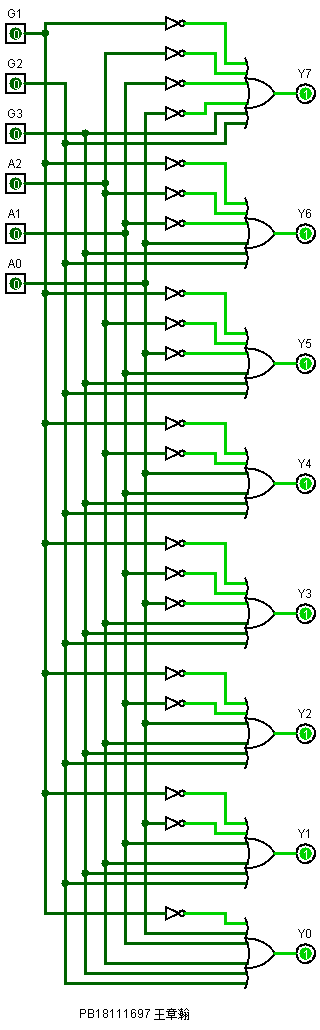
\includegraphics[scale=0.5]{Problem2.png}
		\caption{题目2的实验结果}
		\label{Problem2}
	\end{figure}\par


	\subsection{题目3}
	\subsubsection{题目}
	使用Logisim绘制1bit位宽的二选一选择器电路图,并根据生成的电路图编写Verilog代码。输入信号为a,b,sel,输出信号为out,sel为0时选通a信号。\par
	\subsubsection{实验结果}
	使用Logisim绘制的1bit位宽二选一选择器电路图如下:\par
	\begin{figure}[h]
		\centering
		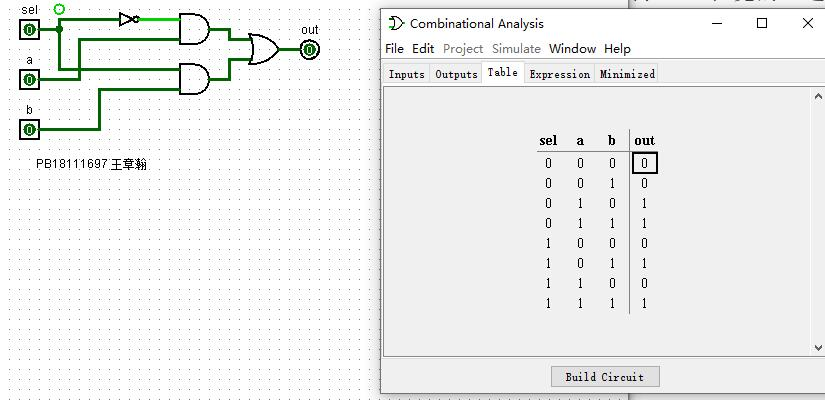
\includegraphics[scale=0.6]{Problem3_Curcuit.jpg}
		\caption{题目3的二选一选择器电路图}
		\label{Problem3_Curcuit}
	\end{figure}\par
	编写的Verilog代码如下:\par
	\begin{lstlisting}[language=Verilog]
	module mux2_1bit(
		input a, b, sel,
		output out);
		assign out = (~sel&a)|(sel&b);
	endmodule
	\end{lstlisting}\par

	\subsection{题目4}
	\subsubsection{题目}
	通过例化题目 3 中的二选一选择器,用Verilog实现一个四选一选择器,并画出对应的电路图。 输入信号为a,b,c,d,sel1, sel0,out,sel1和sel0都为0时选中a信号。\par
	\subsubsection{实验结果}
	编写的Verilog代码如下:\par
	\begin{lstlisting}[language=Verilog]
	module mux4_1bit(
		input a,
		input b,
		input c,
		input d,
		input sel1,
		input sel0,
		output out
		);
		wire temp0, temp1;
		mux2_1bit mux2_inst1(
			.a(a),
			.b(b),
			.sel(sel0),
			.out(temp0));
		mux2_1bit mux2_inst2(
			.a(c),
			.b(d),
			.sel(sel0),
			.out(temp1));
		mux2_1bit mux2_inst3(
			.a(temp0),
			.b(temp1),
			.sel(sel1),
			.out(out));
	endmodule
	\end{lstlisting}\par
	利用Vivado的仿真功能枚举所有情况,得到如下图:\par
	\begin{figure}[H]
		\centering
		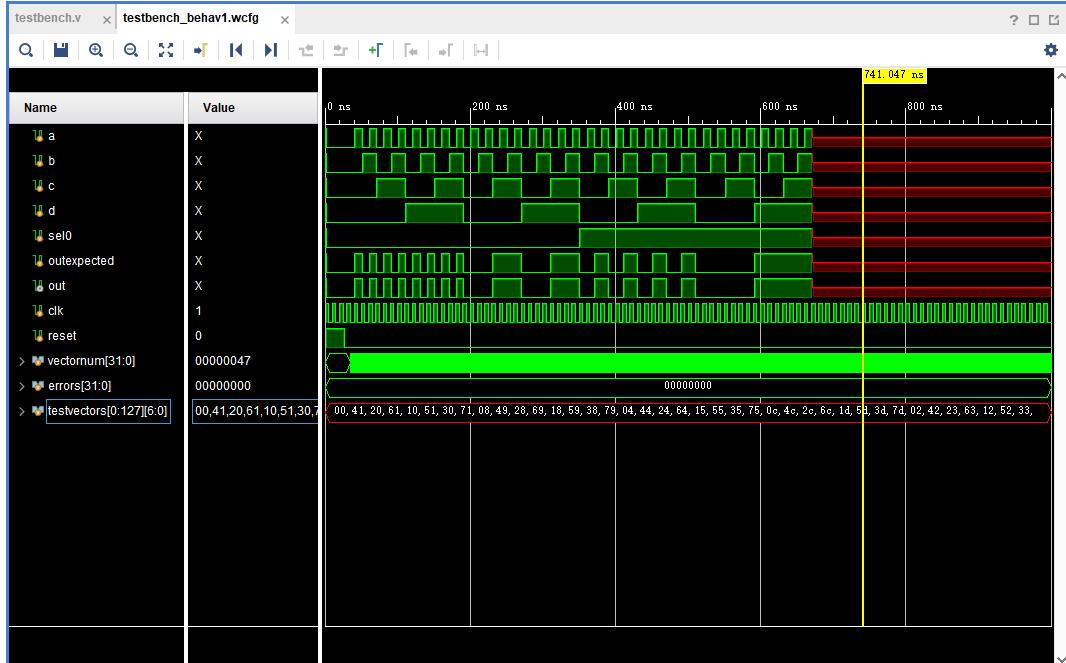
\includegraphics[scale=0.5]{Problem4_Mux4_1bit_Simulation.jpg}
		\caption{题目4的Vivado仿真结果}
		\label{Problem4_Mux4_1bit_Simulation}
	\end{figure}\par
	这说明该代码是正确的。\par
	此外,其相应的电路图如下:
	\begin{figure}[H]
		\centering
		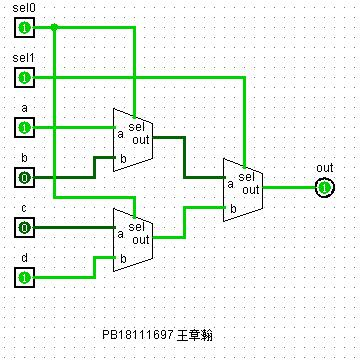
\includegraphics[scale=1]{Problem3_Mux4_1bit.jpg}
		\caption{题目4的四选一选择器电路图}
		\label{Problem3_Mux4_1bit}
	\end{figure}\par

	\subsection{题目5}
	\subsubsection{题目}
	根据前面用到的八位优先编码器真值表,编写 verilog 代码。\par
	\subsubsection{实验结果}
	经过Logisim辅助进行简化,得到如下表达式:\par
	\begin{center}
		$y0 = \overline{i6}\  \overline{i4}\ \overline{i2}\ i1\ +\ \overline{i6}\ \overline{i4}\ i3\ +\ \overline{i6}\ i5\ +\ i7$\\
		$y1 = \overline{i5}\ \overline{i4}\ i2\ +\ \overline{i5}\ \overline{i4}\ i3\ +\ i6\ +\ i7$\\
		$y2 = i4\ +\ i5\ +\ i6\ +\ i7$\\
	\end{center}\par
	据此编写Verilog代码如下:\par
	\begin{lstlisting}[language=Verilog]
	module encoder(
		input [7:0] i,
		output [3:0] y
		);
		assign y[0] = (~i[6] & ~i[4] & ~i[2] & i[1]) 
			| (~i[6] & ~i[4] & i[3]) 
			| (~i[6] & i[5]) 
			| i[7];
		assign y[1] = (~i[5] & ~i[4] & i[2]) 
			| (~i[5] & ~i[4] & i[3]) 
			| i[6] 
			| i[7];
		assign y[2] = i[4] | i[5] | i[6] | i[7];
	endmodule
	\end{lstlisting}\par
	
	\subsection{题目6}
	\subsubsection{题目}
	阅读如下 Verilog 代码,描述其功能,并画出其对应的电路
	图。
	\begin{lstlisting}[language=Verilog]
	module test(
		input a,b,c,
		output s1,s2);
		assign s1= ~a &~b & c + ~a & b &~c + a &~b &~c + a & b & c;
		assign s2= ~a & b & c + a &~b & c + a & b &~c + ~a &~b &~c;
	endmodule
	\end{lstlisting}\par
	\subsubsection{实验结果}
	可以看出来,s1和s2的表达式如下:
	\begin{center}
		$s1 = \overline{a}\ \overline{b}\ c\ \oplus\ \overline{a}\ b\ \overline{c}\ \oplus\ a\ \overline{b}\ \overline{c}\ \oplus\ a\ b\ c$\\
		$s1 = \overline{a}\ b\ c\ \oplus\ a\ \overline{b}\ c\ \oplus\ a\ b\ \overline{c}\ \oplus\ \overline{a}\ \overline{b}\ \overline{c}$\\
	\end{center}\par
	其电路图如下:
	\begin{figure}[H]
		\centering
		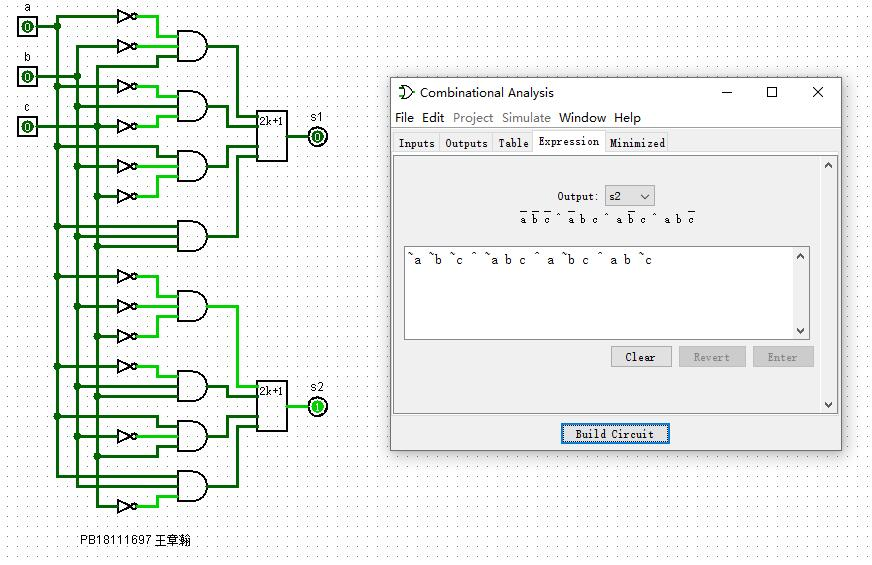
\includegraphics[scale=0.6]{Problem6_Curcuit_Complex.jpg}
		\caption{题目6未简化电路图}
		\label{Problem6_Curcuit_Complex}
	\end{figure}\par
	借助Logisim的表达式化简功能,可以知道上式实际上如下:
	\begin{center}
		$s1 = \overline{a}\ \overline{b}\ c\ +\ \overline{a}\ b\ \overline{c}\ +\ a\ \overline{b}\ \overline{c}\ +\ a\ b\ c$\\
		$s1 = \overline{a}\ b\ c\ +\ a\ \overline{b}\ c\ +\ a\ b\ \overline{c}\ +\ \overline{a}\ \overline{b}\ \overline{c}$\\
	\end{center}\par
	可以画出电路图:
	\begin{figure}[H]
		\centering
		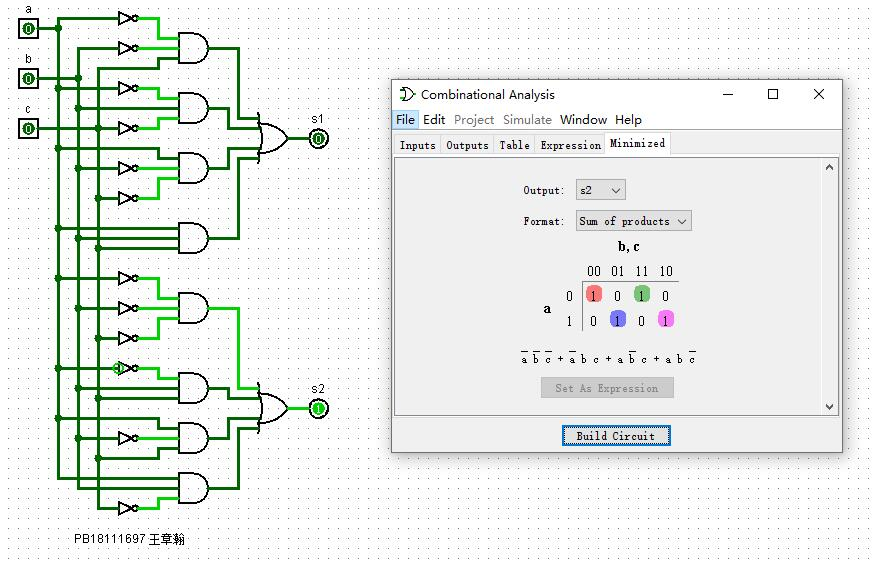
\includegraphics[scale=0.6]{Problem6_Curcuit.jpg}
		\caption{题目6简化后电路图}
		\label{Problem6_Curcuit}
	\end{figure}\par
	由此容易看出来,题述Verilog代码实现的功能是统计输入a,b,c值为1的个数的奇偶性。若为个数为奇数,则s1=1,s2=0;若为偶数,则s1=0,s2=1\par
	\section{总结与思考}
	
	\subsection{本次实验的收获}
	在本次实验中,我进一步了解了Logisim的高阶操作。能够使用Logisim中利用真值表,表达式来画电路图,并利用相关功能化简表达式,使得利用Logisim的效率更高。此外,也初步接触了Verilog代码的使用,了解了Verilog模块的基本结构与基本使用方法,包括input,output的使用,wire的含义,assign的使用等。\par
	
	\subsection{评价本次实验的难易程度}
	本次实验内容难度适中,基本上是可以自主完成的。\par
	
	\subsection{评价本次实验的任务量}
	本次实验任务量较大,需要课后花费五、六个小时才能完成。但这可能是刚开始接触相关实验还不能较好适应导致的。\par
	
	\subsection{为本次实验提供改进建议}
	本次实验的实验指导书中有涉及到表达式的内容。其中,模数课程上表达式使用的或所用符号是+,而Verilog中的+表示的是加法,对于单bit数据来说,相当于一个异或的操作。这一点容易引起不清,还望详述。此外,如能将Verilog的介绍放在Vivado使用的解说之后,可能效果更好。
	
\end{document}
